\documentclass[tikz,border=10pt]{standalone}
\begin{document}
% Scale from STYLE METRICS: s = 0.021333 cm/px (longest side 375 px -> 8 cm)
% x_t = (px - 224.26)*s, y_t = (201.13 - py)*s
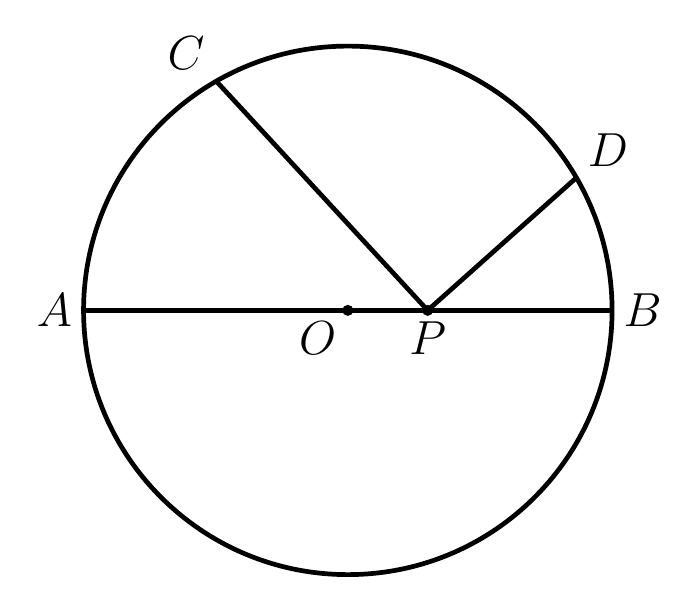
\begin{tikzpicture}[line join=round, line width=1.7pt]

% Named coordinates (cm)
\coordinate (O) at (0,0);
\coordinate (A) at (-3.356,0);   % circle radius 157.3 px -> 3.356 cm
\coordinate (B) at (3.356,0);
\coordinate (P) at (1.014,0);
\coordinate (C) at (-1.671,2.911);
\coordinate (D) at (2.903,1.685);

% Circle (centre O, radius 3.356 cm)
\draw (O) circle[radius=3.356];

% Diameter AB
\draw (A) -- (B);

% Segments CP and PD
\draw (C) -- (P) -- (D);

% Small filled dots at O and P only
\fill (O) circle[radius=2pt];
\fill (P) circle[radius=2pt];

% Labels (font from STYLE METRICS)
\node[font=\fontsize{17}{20.4}\selectfont, left] at (A) {$A$};
\node[font=\fontsize{17}{20.4}\selectfont, right] at (B) {$B$};
\node[font=\fontsize{17}{20.4}\selectfont, below left] at (O) {$O$};
\node[font=\fontsize{17}{20.4}\selectfont, below] at (P) {$P$};
\node[font=\fontsize{17}{20.4}\selectfont, above left] at (C) {$C$};
\node[font=\fontsize{17}{20.4}\selectfont, above right] at (D) {$D$};

\end{tikzpicture}
\end{document}